%% ------------------------------------------------------------------
%% FEATURE - project report (JMLR format)
%%
%% Requires jmlr2e.sty (the official JMLR style file). It ships with the
%% JMLR template on Overleaf and can also be downloaded from
%% https://www.jmlr.org/format/ . If it is not found, this file falls back
%% to a self-contained approximation so it still compiles. Run pdflatex
%% twice for the references.
%%
%% Figures live in ./figures/ (copied from results/<run>/).
%% ------------------------------------------------------------------
\documentclass[twoside,11pt]{article}

\IfFileExists{jmlr2e.sty}{%
  \usepackage{jmlr2e}
}{%
  \usepackage[margin=1in]{geometry}
  \usepackage{natbib}
  \newcommand{\ShortHeadings}[2]{}
  \newcommand{\firstpageno}[1]{\setcounter{page}{##1}}
  \newcommand{\editor}[1]{}
  \newcommand{\name}{}
  \newcommand{\email}[1]{\texttt{##1}}
  \newcommand{\addr}{}
  \newenvironment{keywords}{\par\medskip\noindent\textbf{Keywords:} }{\par}
}
\usepackage{booktabs}
\usepackage{amsmath}
\usepackage{graphicx}

\ShortHeadings{Language-Independence of Phonological Features in wav2vec 2.0}{}
\firstpageno{1}

\begin{document}

\title{Do Self-Supervised Speech Models Encode Phonological Features
Language-Independently? A Probing Study of wav2vec 2.0 Variants}

\author{\name Muhammad Haider Zaidi \email haider.zaidi@fau.de \\
        \addr Biomedical Image Analysis Project}

\editor{}

\date{24 July 2026}

\maketitle

% ==================================================================
\begin{abstract}
Self-supervised speech models such as wav2vec 2.0 learn strong representations
from raw audio and are known to encode substantial phonetic information. I study
whether they encode phonological features (voicing, nasality, manner and place of
articulation) as language-independent properties, and whether languages share
this latent structure. I probe three wav2vec 2.0 variants, a monolingual base
model and two multilingual XLSR models, on English, German and Spanish (FLEURS),
training linear probes on phoneme-level representations obtained by MMS forced
alignment, and I evaluate three hypotheses across models (H1), layers (H2) and
features (H3). Phonological information peaks in the upper-middle layers (about
70 to 75\% of network depth) and declines toward the top, consistently across
models (H2). Multilingual models hold a modest but consistent cross-lingual
advantage over the monolingual baseline (H1). Features differ sharply in
transferability: nasality's cross-lingual gap is statistically indistinguishable
from zero, while manner of articulation shows the largest and clearly significant
gap (H3). Transfer between all language pairs is broadly symmetric. Underlying
these results, replacing uniform frame assignment with forced alignment roughly
doubled probe accuracy, which shows that accurate phoneme to frame alignment is
essential for this analysis.
\end{abstract}

\begin{keywords}
  self-supervised speech representations, wav2vec 2.0, probing, phonological
  features, cross-lingual transfer, forced alignment
\end{keywords}

% ==================================================================
\section{Introduction}

Self-supervised speech models such as wav2vec 2.0 have become important
foundations for speech processing because they learn strong representations
directly from raw waveform audio. I'm working with three models here: the base
wav2vec 2.0 model, and two multilingual variants, XLSR-53, which was trained on 53
languages, and XLS-R, a 300-million-parameter model trained on 128 languages.
Prior probing work suggests that the embeddings of these models encode phonetic
and phonological information. In this research I aim to understand how that
information is organised in the model and across different languages.

Even though we know these models capture phonetic information, it's still not
clear whether they encode phonological features as language-independent concepts,
or whether they just learn each language on its own. It's also unclear whether
different languages end up sharing the same underlying phonological structure
inside the model. These are the gaps I'm looking into.

This matters for a couple of reasons. First, it helps us understand what these
black-box speech models are actually learning about speech sounds. Second, if
phonology is encoded in a universal way, then a model trained on one language
should transfer to another, which is useful for low-resource languages that don't
have a lot of data. It also tells us whether multilingual pretraining is really
worth it when the task is phonological.

I'm trying to answer these questions with three hypotheses:

\begin{itemize}
  \item \textbf{H1:} multilingual models encode phonology more
        language-independently than monolingual ones, and therefore they have
        better cross-lingual transfer.
  \item \textbf{H2:} the middle layers of the model tend to encode the
        phonological information.
  \item \textbf{H3:} some of these features (voicing, nasality, place of
        articulation, and manner of articulation) transfer well across languages,
        while others are more language-specific.
\end{itemize}

To answer these questions, I extract the hidden representations from every layer
of the three models, for English, German and Spanish speech from the FLEURS
dataset. I then align each phoneme to its audio frames using forced alignment, and
train a simple linear probe to predict each phonological feature from the
representation. I check how well the probe transfers across languages, and I use
cross-validation and confidence intervals so the results are statistically
grounded and not just single numbers.

% ==================================================================
\section{Related Work}

Self-supervised speech models like wav2vec 2.0 \citep{baevski2020wav2vec} learn
representations from raw audio without labels, and they have become a common
starting point for speech tasks. The multilingual versions, XLSR-53
\citep{conneau2021xlsr} and XLS-R \citep{babu2022xlsr}, train on many languages at
once and transfer well across them, at least for speech recognition.

Probing is a common way to check what a neural representation has actually
learned. The idea is to train a simple classifier on top of a frozen model and see
if it can recover some property of interest. \citet{hewitt2019control} point out
that a probe can sometimes memorize rather than reveal real structure, and they
suggest control tasks to check for this.

For speech models specifically, earlier work has shown that wav2vec 2.0 embeddings
contain a lot of phonetic and phonological information. \citet{pasad2021layerwise}
did a layer-wise analysis and found that this information is not spread evenly
through the network, and that the layers follow an autoencoder-like pattern where
the middle layers carry the most phonetic detail.

Most of this work looks at a single language, or at phonetic information in
general. What I add here is a direct comparison between a monolingual and two
multilingual models, a per-feature look at how well phonology transfers across
languages, and confidence intervals so the comparisons are backed by statistics
and not just single numbers.

% ==================================================================
\section{Background}

\subsection{wav2vec 2.0}
wav2vec 2.0 learns from raw audio without any labels. It has two parts: a
convolutional feature encoder that turns the waveform into a sequence of frames,
and a Transformer on top that adds context across those frames. It is trained by
masking parts of the audio and learning to predict them, in a contrastive way where
the model has to pick the correct piece out of a set of distractors. Because the
training only uses the audio itself and no transcripts, the model has to discover
useful structure on its own, and this is where the phonetic information is thought
to come from. The output is one vector per frame at each layer, with about 50 frames
per second. The multilingual variants I use, XLSR-53 and XLS-R, work the same way
but are trained on many languages at once, which is meant to give them
representations that work across languages.

\subsection{Phonological features}
Phonological features describe how a speech sound is physically produced, rather
than what it means or how it is spelled. I look at four of them. Voicing is whether
the vocal cords vibrate, which separates sounds like b, d, z from p, t, s.
Nasality is whether air comes out through the nose, as in m, n, and ng. Manner of
articulation is how the airflow is obstructed, going from a full block (plosive) to
a narrow hiss (fricative) to almost no constriction (approximant). Place of
articulation is where in the mouth the constriction happens, from the lips to the
tongue tip to the back of the tongue to the throat. Table~\ref{tab:features} lists
them with examples. The important thing for this project is that these features are
defined the same way in every language, so a nasal is a nasal whether the language
is English, German, or Spanish. That is exactly what makes them a good test of
whether the model has learned phonology in a language-independent way.

\begin{table}[t]
\centering
\begin{tabular}{lll}
\toprule
feature & classes & examples \\
\midrule
voicing & voiced, voiceless & voiced: b, d, z \quad voiceless: p, t, s \\
nasal   & nasal, oral & nasal: m, n, ng \quad oral: all other sounds \\
manner  & plosive, fricative, affricate, & p (plosive), s (fricative), \\
        & nasal, approximant & ch (affricate), m (nasal), l (approximant) \\
place   & labial, coronal, dorsal, laryngeal & p (labial), t (coronal), \\
        &  & k (dorsal), h (laryngeal) \\
\bottomrule
\end{tabular}
\caption{The four phonological features, their classes, and example sounds. Each
feature is only probed on the segments where it is contrastive: voicing on
obstruents, manner and place on consonants, and nasal on all segments.}
\label{tab:features}
\end{table}

\subsection{Linear probing}
To measure whether the model encodes a feature, I train a simple linear classifier
(a probe) on top of the frozen representation and check if it can predict the
feature. If a linear probe can recover the feature, then the model must have
encoded it in a clear, linearly readable way. I keep the probe linear on purpose,
because a more powerful probe could find structure that the model did not actually
expose, which would make the result harder to interpret. Figure~\ref{fig:probe}
shows the idea: each point is a phoneme's representation, and the probe learns a
boundary that separates the classes.

\begin{figure}[t]
  \centering
  
\includegraphics[width=0.72\textwidth]{figures/probe_illustration.png}
  \caption{What a linear probe does, illustrated for voicing in two dimensions
  (the real representation has 768 dimensions). Each point is one phoneme; the
  probe learns a straight boundary that separates the classes. If the classes are
  linearly separable, the feature is encoded in a readable way.}
  \label{fig:probe}
\end{figure}

\subsection{Evaluating a probe}
The labels are not balanced. For voicing, for example, there are more voiceless
obstruents than voiced ones, so a classifier that always guesses the majority class
would already get a decent accuracy without learning anything. To avoid being
fooled by this, I report macro-F1, which is the F1 score averaged over the classes
so that each class counts equally, no matter how rare it is. I always compare the
probe against a majority-class baseline, which is what you would get by always
predicting the most common label, and I compute that baseline as macro-F1 too so it
is on the same scale as the probe. A probe is only interesting if it clearly beats
this baseline.

One more thing matters for a fair evaluation. Phonemes that come from the same
recording are not independent, since they share the same speaker and the same
audio. If I split the phonemes randomly, some phonemes from a recording could end up
in training and others in testing, and the probe could get a good score just by
recognizing the recording rather than the phonology. To prevent this I group the
split by utterance, so all the phonemes from one recording stay on the same side of
the split.

\subsection{Forced alignment}
The model produces frames, but the labels are phonemes, so I need to know which
frames belong to which phoneme. Forced alignment solves this: given the audio and
the transcript, which I already have, it finds where each word occurs in time.
This is different from speech recognition, which tries to guess the words. Here the
words are already known, and I only need their timing.

% ==================================================================
\section{Methods}

The pipeline has four steps, shown in Figure~\ref{fig:pipeline}. I extract the
hidden states from the models, turn the transcriptions into phonological labels,
align the labels to the representations and train the probes, and then analyse the
scores to answer the three hypotheses. The rest of this section describes each step.

\begin{figure}[h]
  \centering
  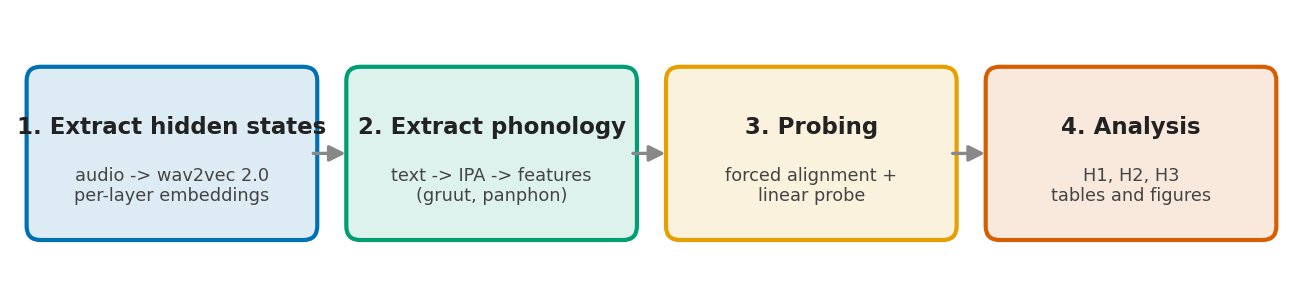
\includegraphics[width=\textwidth]{figures/pipeline.png}
  \caption{The four steps of the pipeline: extracting hidden states from the
  models, extracting phonological labels from the text, probing (which includes
  forced alignment and the linear probe), and the final analysis.}
  \label{fig:pipeline}
\end{figure}

\subsection{Data}
I use the FLEURS dataset, which is a multilingual read-speech corpus. I work with
three languages: English (en\_us), German (de\_de), and Spanish (es\_419), and I
use 100 utterances per language at 16 kHz. FLEURS is parallel, which means the
same sentences are translated across all the languages, so the three languages
cover the same content and there's no topic bias between them. The actual words
and phonemes are still different in each language though, since they are
translations of each other.

From these utterances I get 8{,}766 phonemes for English, 11{,}952 for German, and
11{,}564 for Spanish. The number of phonemes each probe actually uses depends on
its segment filter, since each feature is only probed on the segments where it is
contrastive. Table~\ref{tab:datastats} shows how many phonemes are kept for each
feature and language. Nasal uses every phoneme, so it has the most data, while
voicing uses only obstruents and so has the least. The classes are also not
balanced, for example there are more voiceless than voiced obstruents and far more
oral than nasal segments, which is exactly why I use macro-F1 and a majority
baseline rather than plain accuracy. The affricate class in manner is especially
rare (fewer than 200 phonemes in total), which makes manner the hardest feature to
probe.

\begin{table}[t]
\centering
\begin{tabular}{lcccc}
\toprule
feature & en\_us & de\_de & es\_419 & total \\
\midrule
voicing (obstruents) & 3{,}225 & 4{,}378 & 3{,}895 & 11{,}498 \\
nasal (all segments)  & 8{,}766 & 11{,}952 & 11{,}564 & 32{,}282 \\
manner (consonants)   & 5{,}220 & 7{,}137 & 6{,}527 & 18{,}884 \\
place (consonants)    & 5{,}220 & 7{,}137 & 6{,}527 & 18{,}884 \\
\bottomrule
\end{tabular}
\caption{Number of phonemes used to probe each feature, per language, after the
segment filter is applied. Nasal is probed on all segments, voicing only on
obstruents, and manner and place only on consonants.}
\label{tab:datastats}
\end{table}

\subsection{Models}
I compare three wav2vec 2.0 variants. The base model is monolingual and trained
only on English, with 12 transformer layers and a hidden size of 768. XLSR-53 is
multilingual, trained on 53 languages, with 24 layers and a hidden size of 1024.
XLS-R is also multilingual, trained on 128 languages, with the same 24 layers and
hidden size of 1024. The base model is my monolingual baseline for the H1
comparison.

\subsection{Extracting hidden states}
I run each model on the utterances without any fine-tuning, so the models stay
frozen. For every utterance I keep the output of every layer, not just the last
one, because H2 is about finding which layer encodes the phonological information.
Each layer gives a grid of shape $(T, D)$, where $T$ is the number of time frames
(about 50 per second, so one frame every 20 ms) and $D$ is the hidden size (768 or
1024).

\subsection{Extracting phonology}
To get the labels, I convert each transcription into phonemes in two steps. First,
gruut does the grapheme-to-phoneme conversion, turning the text into IPA. Then
panphon \citep{mortensen2016panphon} maps each IPA symbol to its distinctive
features. I collapse those into four labels: voicing (voiced or voiceless), nasal
(nasal or oral), manner (plosive, fricative, affricate, nasal, or approximant),
and place (labial, coronal, dorsal, or laryngeal).

Each feature is only probed on the segments where it actually means something.
Voicing is probed on obstruents only, because sonorants are almost always voiced,
so probing it on everything would give a nearly constant label. Manner and place
are probed on consonants only, since they are undefined for vowels. Nasal is
probed on all segments.

\subsection{Aligning phonemes to frames}
To attach the labels to the representations, I need to know which audio frames
belong to which phoneme. I use the MMS forced aligner \citep{pratap2024mms} to get
word-level time spans, which tell me where each word occurs in the audio. I then
split each word's time span evenly across its phonemes to get a time span for each
phoneme. Each phoneme's time span is converted into frame indices using the clip
duration, and I mean-pool the frames inside that span into a single vector. This
gives me one representation per phoneme, paired with its label. This replaced an
earlier version that just split the whole utterance evenly across all its
phonemes, which was a lot less accurate.

\subsection{Probing}
For each combination of model, feature, layer, and language, I train a linear
probe (logistic regression) to predict the label from the phoneme vector. I
standardize the features first. I keep the probe linear on purpose, because that
tests whether the feature is linearly readable from the representation, so the
probe can't invent structure that the model didn't actually expose. I report
macro-F1, since the labels are imbalanced and plain accuracy would be misleading,
and I compare it against a majority-class baseline that is also computed as
macro-F1. The train and test splits are grouped by utterance, so phonemes from the
same recording never end up on both sides, which avoids leakage. I repeat this
over 5 grouped splits and report the mean and standard deviation.

\subsection{Cross-lingual transfer and statistics}
For the cross-lingual part, I do zero-shot transfer: I train the probe on one
language and test it on the others, covering all the ordered language pairs. I
report transfer at each model and feature's best layer, chosen by within-language
macro-F1, so I'm not picking an arbitrary layer.

For H3, I measure the transfer gap, which is the within-language macro-F1 minus the
cross-lingual macro-F1. I use a paired $k$-fold procedure: I split language A's
utterances into 5 folds, repeated 3 times, and in each fold I train one probe and
test it both on the held-out utterances of A (within) and on the other languages
(cross). Because both scores come from the same probe and training set, the gap is
paired. This gives 45 gap estimates per model and feature, and I report the mean
and a 95\% confidence interval from the percentiles. I treat a gap as real if its
confidence interval excludes zero. I also compute the paired differences between
features on the same folds. I use a percentile confidence interval rather than a
standard t-test, because the folds share most of their training data and so their
scores are correlated, which would make a t-test overconfident.

% ==================================================================
\section{Results}

The results in this section improved a lot over the course of the project, and it
is worth showing this because it makes clear how much the method matters. My first
complete run used uniform alignment, splitting each utterance's frames evenly
across its phonemes. The scores were weak and flat: within-language voicing only
reached about 0.54 and manner about 0.22, barely above their baselines, so it
looked like the models were not encoding much. Replacing uniform splitting with MMS
forced alignment was the turning point. Lining each phoneme up with the frames it
actually occupies roughly doubled the scores, for example within-language voicing
went from about 0.54 to 0.85 and manner from about 0.22 to 0.67
(Table~\ref{tab:align}). The models and the probes were exactly the same, so the
improvement came entirely from better alignment, which showed that the earlier weak
results were a measurement problem and not a real absence of phonological
information. A final round of work on grouped splits, error bars, best-layer
selection and the paired $k$-fold test did not raise the numbers, but it made them
trustworthy. All the results below use forced alignment.

\begin{table}[t]
\centering
\begin{tabular}{lccc}
\toprule
feature & uniform alignment & forced alignment & change \\
\midrule
voicing & 0.54 & 0.85 & $+0.31$ \\
nasal   & 0.47 & 0.76 & $+0.29$ \\
place   & 0.34 & 0.77 & $+0.43$ \\
manner  & 0.22 & 0.67 & $+0.45$ \\
\bottomrule
\end{tabular}
\caption{Effect of alignment on within-language decodability (best within-language
macro-F1, base model). Switching from uniform to MMS forced alignment roughly
doubled every feature, using the same models and probes.}
\label{tab:align}
\end{table}

\subsection{H2: which layers encode phonology}
Figure~\ref{fig:h2} shows the macro-F1 of each feature at each layer. All four
features are well above their baselines at every layer, so the phonological
information is decodable through the whole network. But the curves are not flat.
They start lower at the input, rise up, peak in the upper-middle layers, and then
drop off again toward the top. For the base model the peak is around layers 8 to
10 out of 12, and for the two larger models it is around layers 16 to 18 out of
24. In both cases that is roughly 70 to 75\% of the way through the network, and
this is consistent across all three models. The features also keep the same order
at almost every layer: voicing is the easiest to decode, place and nasal sit close
together in the middle, and manner is the hardest. The drop in the top layers
makes sense, since those layers tend to specialize back towards the model's own
pretraining objective. Overall this supports H2.

\begin{figure}[t]
  \centering
  
\includegraphics[width=\textwidth]{figures/fig_h2_layers.png}
  \caption{H2: macro-F1 by layer for each model (mean over languages, shaded
  band is $\pm 1$ standard deviation across languages). All features peak in the
  upper-middle layers and decline toward the top.}
  \label{fig:h2}
\end{figure}

\subsection{H1: multilingual vs monolingual}
Table~\ref{tab:h1} shows the cross-lingual transfer for each model, measured at
each feature's best layer. The two multilingual models match or beat the
monolingual base model on every feature. The biggest differences are on voicing,
where base gets 0.67 and XLS-R gets 0.75, and on manner, where base gets 0.45 and
XLS-R gets 0.53. But most of these differences are small, often around the same
size as the bootstrap standard deviation of about 0.04, so the advantage is
consistent in direction but not very large. So H1 is only partly supported: for
these three related languages, multilingual pretraining does give a cross-lingual
benefit, but a modest one.

\begin{table}[t]
\centering
\begin{tabular}{lcccc}
\toprule
feature & base & XLSR-53 & XLS-R & majority baseline \\
\midrule
voicing & 0.667 & 0.721 & \textbf{0.753} & 0.38 \\
nasal   & 0.720 & \textbf{0.760} & 0.728 & 0.47 \\
place   & 0.628 & \textbf{0.660} & 0.658 & 0.26 \\
manner  & 0.452 & 0.513 & \textbf{0.533} & 0.09 \\
\bottomrule
\end{tabular}
\caption{H1: cross-lingual transfer macro-F1 (all language pairs, at the best
layer). Bootstrap standard deviations are about 0.04.}
\label{tab:h1}
\end{table}

Figure~\ref{fig:h1bars} shows the same comparison as a bar chart, which makes the
small size of the differences easier to see. The multilingual models are usually a
little ahead, but the bars are close and the error bars overlap for most features,
which is why I describe the advantage as consistent but modest.

\begin{figure}[t]
  \centering
  
\includegraphics[width=\textwidth]{figures/fig_h1_models.png}
  \caption{H1: cross-lingual transfer macro-F1 per feature, grouped by model, at
  the best layer. The multilingual models are usually slightly ahead of base, but
  the differences are small.}
  \label{fig:h1bars}
\end{figure}

I also checked whether the model differences depend on the layer, by looking at
cross-lingual transfer at every layer rather than only the best one
(Figure~\ref{fig:h1layer}). The models track each other closely at every depth, so
the modest multilingual advantage is not something that only appears at one lucky
layer, it holds across the network.

\begin{figure}[t]
  \centering
  
\includegraphics[width=\textwidth]{figures/fig_h1_transfer_by_layer.png}
  \caption{Cross-lingual transfer by layer for each model. The models follow
  similar curves at every depth, with the multilingual models usually slightly
  ahead, so the advantage is not tied to any particular layer.}
  \label{fig:h1layer}
\end{figure}

\subsection{H3: which features transfer across languages}
Figure~\ref{fig:h3} shows the transfer gap for each feature with its 95\%
confidence interval, where the gap is the within-language score minus the
cross-lingual score. A gap is only real if its confidence interval stays above
zero. Manner has the largest gap in every model, around 0.21 to 0.24, and it is
clearly significant, so it is the most language-specific feature. Nasal is the
opposite: its gap is small (0.03 to 0.07) and its confidence interval includes
zero in all three models, so its gap is statistically indistinguishable from zero.
In other words nasality transfers across languages essentially for free. Voicing
is significant in all three models, and place is significant in two of them and
borderline in the third. The important part is that the ranking, manner then
voicing and place then nasal, is identical across all three models, which suggests
it reflects a property of phonology itself and not just one model. The paired test
also confirms that the difference between manner and nasal is significant in every
model. This supports the core of H3, but not my original guess that place would be
the most language-specific feature, since that turned out to be manner, and nasal
turned out to be the most universal.

\begin{figure}[t]
  \centering
  
\includegraphics[width=\textwidth]{figures/fig_h3_gap_ci.png}
  \caption{H3: transfer gap (within-language minus cross-lingual macro-F1) with
  95\% confidence intervals. Blue means the interval excludes zero (a real gap);
  grey means it includes zero (indistinguishable from language-independent).
  Nasal is grey in all models; manner shows the largest gap.}
  \label{fig:h3}
\end{figure}

The same result can be seen in a more intuitive way in Figure~\ref{fig:h3std},
which plots the within-language and cross-lingual scores side by side with a band
for their spread across the k-fold splits. When the two bands overlap, the gap is
within the noise, and when they are clearly apart, the gap is real. For nasal the
two bands sit almost on top of each other, while for manner they are far apart.
This is the same conclusion as the confidence intervals, just shown visually.

\begin{figure}[t]
  \centering
  
\includegraphics[width=\textwidth]{figures/fig_h3_gap_std.png}
  \caption{H3 shown as within-language versus cross-lingual scores, with bands for
  the spread across k-fold splits. Overlapping bands mean the gap is not real
  (nasal); clearly separated bands mean it is (manner).}
  \label{fig:h3std}
\end{figure}

Finally, I tested whether the features are significantly different from each other,
not just from zero. Figure~\ref{fig:h3pair} shows the paired differences between
every pair of features with their confidence intervals. The manner versus nasal
difference is clearly significant in every model, which confirms that manner really
is more language-specific than nasal and this is not just noise.

\begin{figure}[t]
  \centering
  
\includegraphics[width=\textwidth]{figures/fig_h3_pairwise.png}
  \caption{H3: paired differences between feature gaps, with 95\% confidence
  intervals. Green means the two features differ significantly (interval excludes
  zero). The manner versus nasal difference is significant in all models.}
  \label{fig:h3pair}
\end{figure}

Table~\ref{tab:h3full} collects the full numbers behind these figures: for every
model and feature it gives the best layer, the within-language and cross-lingual
scores, the transfer gap, its 95\% confidence interval, and whether the gap is
significant. The pattern is consistent across models. Nasal is never significant,
manner and voicing are always significant, and place is significant for two of the
three models and just borderline for the third (its lower bound is almost exactly
zero).

\begin{table}[t]
\centering
\small
\begin{tabular}{llccccc}
\toprule
model & feature & best layer & within & cross & gap [95\% CI] & significant \\
\midrule
base & voicing & 10 & 0.848 & 0.667 & 0.182 [0.128, 0.254] & yes \\
base & nasal   & 10 & 0.755 & 0.720 & 0.035 [$-$0.083, 0.132] & no \\
base & place   & 6  & 0.765 & 0.628 & 0.136 [0.044, 0.209] & yes \\
base & manner  & 8  & 0.668 & 0.452 & 0.215 [0.113, 0.305] & yes \\
\midrule
XLSR-53 & voicing & 16 & 0.878 & 0.721 & 0.156 [0.114, 0.241] & yes \\
XLSR-53 & nasal   & 16 & 0.795 & 0.760 & 0.035 [$-$0.043, 0.086] & no \\
XLSR-53 & place   & 16 & 0.821 & 0.660 & 0.160 [0.025, 0.232] & yes \\
XLSR-53 & manner  & 16 & 0.747 & 0.513 & 0.235 [0.150, 0.336] & yes \\
\midrule
XLS-R & voicing & 18 & 0.880 & 0.753 & 0.127 [0.081, 0.205] & yes \\
XLS-R & nasal   & 16 & 0.800 & 0.728 & 0.072 [$-$0.059, 0.129] & no \\
XLS-R & place   & 18 & 0.814 & 0.658 & 0.156 [$-$0.002, 0.227] & no \\
XLS-R & manner  & 16 & 0.747 & 0.533 & 0.214 [0.106, 0.306] & yes \\
\bottomrule
\end{tabular}
\caption{Full H3 results per model and feature: best layer, within-language and
cross-lingual macro-F1, the transfer gap with its 95\% confidence interval, and
whether the gap is significant (interval excludes zero). Within-language scores are
also a useful summary of how decodable each feature is.}
\label{tab:h3full}
\end{table}

\subsection{All-pairs transfer}
I also looked at transfer between every pair of languages
(Figure~\ref{fig:langmat}). The matrix is roughly symmetric, so training on any
one of the three languages and testing on the others gives similar scores. This
fits the idea that the three languages share a lot of the same latent
phonological structure.

\begin{figure}[t]
  \centering
  
\includegraphics[width=\textwidth]{figures/fig_language_matrix.png}
  \caption{All-pairs transfer matrix per model (rows are the training language,
  columns are the test language, averaged over features at the best layer). The
  diagonal is within-language performance.}
  \label{fig:langmat}
\end{figure}

% ==================================================================
\section{Discussion}

\paragraph{Alignment turned out to be the most important part.}
The single biggest thing I learned is how much the phoneme to frame alignment
matters. My earlier version just split each utterance's frames evenly across all
its phonemes, which ignored the leading silence and the fact that phonemes have
very different lengths. With that approach the probes were barely above chance.
Once I switched to MMS forced alignment the scores roughly doubled, for example
within-language voicing went from about 0.54 to about 0.85. So phoneme-level
probing of these models is very sensitive to alignment quality, and a bad
alignment can completely hide the structure that is actually there.

\paragraph{What the results mean.}
The layer pattern in H2 fits the usual view that these models build up more
abstract phonetic information in the middle and then specialize the top layers
back towards their pretraining task. This also matches what
\citet{pasad2021layerwise} found in their layer-wise analysis, where the middle
layers carried the most phonetic detail, so it is reassuring to see the same shape
here for phonological features and across three languages rather than just one.

The modest multilingual advantage in H1 probably has a lot to do with the languages
I used. English, German and Spanish are all Indo-European and share most of their
sounds, so even a monolingual English model has already seen most of the phonemes
it needs, and there is not much room left for multilingual pretraining to help. A
bigger advantage might show up for languages that are more different from English.
The feature ranking in H3 makes linguistic sense too: nasality is acoustically
strong and realized in a similar way across languages, while manner covers five
categories with finer differences that vary more between languages.

\paragraph{Limitations.}
The main limitation is the language sample. I only used three languages, and they
are all Indo-European with a lot of overlap in their sounds. So my statistical
tests are valid within English, German and Spanish, and I can say things like
manner transfers worse than nasal in these languages, but I cannot claim that any
feature is universal across all human languages, because for that kind of claim
the real sample size is just three. There are also two smaller limitations. The
alignment is only accurate at the word level, and inside each word I still split
the phonemes evenly, so a phoneme-level aligner would remove that last
approximation. And the best layer for H1 and H3 is chosen on the same data I
report on, though I reduce this problem for H3 by measuring the gap on held-out
folds.

\paragraph{Future work.}
The most useful next step would be to add languages that are very different from
English, like a tonal language or a click language, because that is the real test
of whether these features are universal. A control task \citep{hewitt2019control}
would also help, by checking how much of the probe's score is real signal versus
memorization. And since fine-tuning was part of the original scope but I did not
get to it, fine-tuning the models and repeating the probing would be a natural
extension, especially for H1.

% ==================================================================
\section{Conclusion}

I set out to study whether wav2vec 2.0 and its multilingual variants encode
phonological features as language-independent properties. Using linear probes on
phoneme-level representations from English, German and Spanish, I found that
phonological information is concentrated in the upper-middle layers and drops off
toward the top, and this is consistent across all three models (H2). The
multilingual models are usually a little better than the monolingual base model at
cross-lingual transfer, but the advantage is modest for these related languages
(H1). The features differ clearly in how well they transfer: nasality's transfer
gap is statistically indistinguishable from zero, so it behaves as if it is
language-independent, while manner of articulation has the largest gap and is the
most language-specific (H3). The same ranking of features shows up in all three
models, which suggests it reflects phonology itself rather than any one model.

The clearest practical lesson is about method rather than models. Getting the
phoneme to frame alignment right was what made the difference between results that
looked like noise and results that were clearly meaningful, since forced alignment
roughly doubled the probe scores. Beyond the specific findings, this is a reminder
that for phoneme-level probing of speech models, the alignment step deserves as much
care as the probing itself.

% ==================================================================
\clearpage
\begin{thebibliography}{9}

\bibitem[Babu et al.(2022)]{babu2022xlsr}
A.~Babu, C.~Wang, A.~Tjandra, et al.
\newblock XLS-R: Self-supervised cross-lingual speech representation learning at
scale.
\newblock In \emph{Interspeech}, 2022.

\bibitem[Baevski et al.(2020)]{baevski2020wav2vec}
A.~Baevski, H.~Zhou, A.~Mohamed, and M.~Auli.
\newblock wav2vec 2.0: A framework for self-supervised learning of speech
representations.
\newblock In \emph{Advances in Neural Information Processing Systems (NeurIPS)},
2020.

\bibitem[Conneau et al.(2021)]{conneau2021xlsr}
A.~Conneau, A.~Baevski, R.~Collobert, A.~Mohamed, and M.~Auli.
\newblock Unsupervised cross-lingual representation learning for speech
recognition.
\newblock In \emph{Interspeech}, 2021.

\bibitem[Conneau et al.(2023)]{conneau2023fleurs}
A.~Conneau, M.~Ma, S.~Khanuja, et al.
\newblock FLEURS: Few-shot learning evaluation of universal representations of
speech.
\newblock In \emph{IEEE Spoken Language Technology Workshop (SLT)}, 2023.

\bibitem[Hewitt and Liang(2019)]{hewitt2019control}
J.~Hewitt and P.~Liang.
\newblock Designing and interpreting probes with control tasks.
\newblock In \emph{Empirical Methods in Natural Language Processing (EMNLP)},
2019.

\bibitem[Mortensen et al.(2016)]{mortensen2016panphon}
D.~R. Mortensen, P.~Littell, A.~Bharadwaj, K.~Goyal, C.~Dyer, and L.~Levin.
\newblock PanPhon: A resource for mapping IPA segments to articulatory feature
vectors.
\newblock In \emph{International Conference on Computational Linguistics
(COLING)}, 2016.

\bibitem[Pasad et al.(2021)]{pasad2021layerwise}
A.~Pasad, J.-C. Chou, and K.~Livescu.
\newblock Layer-wise analysis of a self-supervised speech representation model.
\newblock In \emph{IEEE Automatic Speech Recognition and Understanding Workshop
(ASRU)}, 2021.

\bibitem[Pratap et al.(2024)]{pratap2024mms}
V.~Pratap, A.~Tjandra, B.~Shi, et al.
\newblock Scaling speech technology to 1{,}000+ languages.
\newblock \emph{Journal of Machine Learning Research}, 25, 2024.

\end{thebibliography}

% ==================================================================
\appendix
\section{Implementation details}

All experiments were run in Python. The models are loaded from the Hugging Face
Transformers library, and the FLEURS data is loaded from the Hugging Face Datasets
library. The three models are \texttt{wav2vec2-base}, \texttt{wav2vec2-large-xlsr-53}
and \texttt{wav2vec2-xls-r-300m}. The audio is kept at 16 kHz, which is what the
models expect.

For the phonology, I use gruut for grapheme-to-phoneme conversion and panphon for
the distinctive features. Because these are slow, I run them once for all the
utterances and cache the results.

The forced alignment uses the MMS aligner from torchaudio. MMS expects text in a
romanized form using only the letters a to z, but gruut needs the original spelling
to phonemize German and Spanish correctly. I handle this by keeping two versions of
each word: the original spelling, with its accents, is used for phonemization, and a
romanized version is used only for the aligner. The alignment for all utterances is
also computed once and cached.

The probe is a logistic regression from scikit-learn, with a standard scaler in
front of it, a maximum of 2000 iterations, and balanced class weights. Each
within-language score is the mean over 5 repeated grouped splits, where the split is
grouped by utterance. For the H3 gap test I use 5 folds repeated 3 times for each of
the 3 training languages, which gives 45 gap estimates per model and feature, and I
take the 95\% confidence interval from the 2.5th and 97.5th percentiles.

\section{Per-language transfer}

Table~\ref{tab:matrix} gives the full all-pairs transfer for each model, averaged
over features at the best layer. The rows are the training language and the columns
are the test language, so the diagonal is within-language performance and the
off-diagonal entries are cross-lingual transfer. The matrices are close to
symmetric, and the off-diagonal values are fairly similar regardless of which
language is used for training, which supports the idea that the three languages
share a lot of the same phonological structure.

\begin{table}[h]
\centering
\small
\begin{tabular}{llccc}
\toprule
model & train $\backslash$ test & en\_us & de\_de & es\_419 \\
\midrule
base & en\_us & 0.835 & 0.661 & 0.651 \\
base & de\_de & 0.629 & 0.754 & 0.565 \\
base & es\_419 & 0.583 & 0.611 & 0.687 \\
\midrule
XLSR-53 & en\_us & 0.878 & 0.703 & 0.670 \\
XLSR-53 & de\_de & 0.678 & 0.806 & 0.637 \\
XLSR-53 & es\_419 & 0.659 & 0.634 & 0.746 \\
\midrule
XLS-R & en\_us & 0.873 & 0.693 & 0.684 \\
XLS-R & de\_de & 0.679 & 0.808 & 0.604 \\
XLS-R & es\_419 & 0.693 & 0.653 & 0.749 \\
\bottomrule
\end{tabular}
\caption{All-pairs transfer macro-F1 for each model (rows are the training
language, columns are the test language), averaged over features at the best layer.
The diagonal is within-language performance.}
\label{tab:matrix}
\end{table}

\end{document}
